\chapter{Hyperfine Spitting of The Antihydrogen Ground State}
\contentof{This chapter recalls a bit of theory about the energy levels of antihydrogen and focuses on the lines that have been measured at ALPHA. Important to mention the zeeman broadening, since we are working at non-zero field, and the experimental protocol of the measurement. Things to mention are ECR, microwave hardware, magnetic field map. Then a description of the experimental protocol, magnetic field decay}

The hyperfine structure is defined as a small shift (roughly 2000 times smaller than that relative to the fine structure) in the electronic energy level of atoms and molecules. This shift originates from the electromagnetic interaction of the electron magnetic momentum and the magnetic/electric multipole moment of the nucleus. Although the shift is smaller compared the magnitude of the energy level gap and other effects, such as the fine structure of the atoms, it has an important interest in atomic and astrophysics as well as in antimatter studies. From the atomic physics point of view, the transition between the 1s hyperfine levels of hydrogen is an important quantity than has been measured with a remarkable precision of \SI{2}{\milli \hertz} (\cite{bestHFShydrogen}), corresponding to a relative precision of \num{1.4e-12}. In nuclear physics, transitions between hyperfine energy levels offers the possibility of investigating the internal structure of the proton and other nuclei and provide test of QED \cite{Karshenboim:2005iy}. From the astrophysical point of view, the 1s hyperfine splitting corresponds to the \SI{21}{\centi \meter} line, which is transparent to galactic medium and has been extensively used to map hydrogen density of galaxies, galaxy rotation curves, redshit effect \cite{Dickeyarticle} and to test variation of fundamental constants (fine structure constant and g factor of the proton) over time \cite{Khatri_2007}. In the antimatter field, this spectral line can be used to test CPT symmetry, by repeating the same measurement on antihydrogen. Currently, two experiment at the antimatter factory at Cern have the capability to perform this measurement as part of their physics programs: the ASACUSA collaboration \cite{Diermaier:2016fsy}, that aims to measure the hyperfine splitting on a antihydrogen beam (on-flight measurement) and the ALPHA collaboration, which has achieved a measurement on 2017 \cite{ALPHA:2017fsh} and \commento{inserisci la citazione quando viene pubblicata}. The present chapter will give an introduction to the physics underlying the measurement and outline the experimental protocol followed in 2023/2024, that has improved the uncertainty by a factor $\simeq$ 50.
The following derivation follows the approach in \cite[cap.~12]{QuantumMechanics}. Only the case of the hyperfine level of the ground state, which are of particular relevance to this thesis, will be discussed; certain details will be omitted, to not burden the discussion

\section{Hyperfine Structure}
\contentof{This section can contains a brief derivation of the physics behind the hyperfine levels of antihydrogen. Present a brief derivation of the physics}

The hydrogen atom is a bound state of a positron and an antiproton. The base Hamiltonian of this system, neglecting all higher-order terms,  takes the form of $H_0 = \frac{p^2}{2\mu} + V(r)$ where $\mu$ is the reduced mass of the anti-proton//positron system, and $V(r)$ is the central static electromagnetic potential. When considering relativist effects, several high-order terms appears, which are encompassed in the equation\footnote{In the full hamiltonian, $\mu = m_e$ has been used, assuming infinite mass for the proton}:

\begin{equation}
H = m_{e} c^2 + \frac{p^2}{2m_e} + V(r) - \dfrac{p^4}{8 m_{e}^3 c^2} + \frac{1}{2m_{e}^2 c^2} \dfrac{dV(r)}{r dr} L \cdot S + \frac{\hbar^2}{8m_{e}^2 c^2} \Delta V(r) + W_{hf} + ...
\end{equation}

the content of this full hamiltonian can be summarized as:

\begin{itemize}
\item $- \dfrac{p^4}{8 m_{e}^3 c^2}$ correspond to the first relativistic energy correction, and can be easily obtained by expanding in series the relativistic energy $E = c \sqrt{p^2 + m_{e}^{2} c^2}$
\item $+ \frac{1}{2m_{e}^2 c^2} \dfrac{dV(r)}{r dr} L \cdot S$ this is the term responsible of the finite structure of the atoms, and correspond to the coupling of the positron magnetic moment ($M_s = \frac{q S}{m_{e}}$) with its angular momentum $L$ (spin-orbit interaction).
\item  $\frac{\hbar^2}{8m_{e}^2 c^2} \Delta V(r)$ is the Darwin term, that arises when we consider non-local interaction between the electron and the Coulomb field of the nucleus.
\item $W_{hf}$ is the term of the Hamiltonian which describes the hyperfine interaction
\end{itemize}

The first three additional terms causes the fine structure of the atoms, and have all $\alpha^2$ order of magnitude. The term $W_{hf}$ has the following expression:

\begin{equation}
W_{hf} = - \frac{\mu_{0}}{4 \pi} \left( \frac{q}{m_{e} r^3} L \cdot M_{I} + \frac{1}{ r^3} [3(M_s \cdot \hat{n} )( M_I \cdot \hat{n}) - M_{s} \cdot M_{I}] + \frac{8 \pi}{3} M_s \cdot M_{I} \delta(r) \right)
\end{equation}

This expression contains new quantities that weren't introduced before: $M_{I}$ is the magnetic moment of the nucleus, $\hat{n}$ is the unit vector connecting the antiproton to the positron, $\mu_0$ is the magnetic permeability of vacuum. The first term is the equivalent of the spin-orbit interaction considering the nucleus spin, the second term is dipole interaction term and the last term is the Fermi contact term. This additional term in the Hamiltionian is the one causing the hyperfine structure of the levels, and it can be shown (look appendix) that the order of magnitude is 2000 times smaller that the fine structure terms \commento{ricordati di fare i conti in appendice}.
In general, the calculation of all these corrections to the energy levels and the interplay of the various physical effects is complex. However, for the specific case into consideration, numerous simplification of the various terms can be applied, making the calculations easier. For a 1s positron, the angular momentum $ l = 0$, so for the term which explicit depend on $L$

\begin{equation}
 \braket{\psi_{n=1,l=0,m_s,m_I}}  L \cdot S \ket{\psi_{n=1,l=0,m_s,m_I}} = 0
\end{equation}

The other terms, Darwin and the "relativist" term does not depend on either positron $S$ and  antiproton $I$ spin. They only act as a coherent shift of the 4 sub-levels constituting the 1s energy level. Although not important for the following discussion, the shift is equal to (The derivation of this formula is left to the appendix):

\begin{equation}
- \frac{1}{8} m_{e} c^{2} \alpha^{4}
\end{equation}

For $W_{hf}$, the first term depending on $L$ is equal to zero for the same argument used above. The second term, the dipole-dipole interaction, is zero because of the spherical symmetry of the s-wave $\psi_{n=1,l=0,m_s,m_I}$. The only relevant term is the Fermi contact term. This term can be written as:

\begin{equation}
\braket{\psi_{n=1,l=0,m_s,m_I}} \left ( \dfrac{2}{3} \mu_{0} M_{s} M_{I} \delta(r) \right ) \ket{\psi_{n=1,l=0,m_s,m_I}} =  A \braket{m_s,m_I} I \cdot S \ket{m_s, m_I} 
\end{equation}

where $A$ is equal to $ \frac{e^2 g_{p}}{3 \epsilon_0 c^2 m_{e} M_{p}}  \frac{1}{4 \pi} |\psi_{n = 1, l = 0} (r)|$. In the expression, the wave function evaluated at $r = 0$ has appeared in the calculation. This term link the value of the hyperfine splitting to nuclear physics, as the internal structure of the nucleus affects the value of $|\psi_{n = 1, l = 0} (r)|$. \commento{The magnitude of this effect is about 33 part per million, as reported in \cite{Karshenboim:2005iy}}. It's not the goal of this thesis to present the state of the art about the various correction term. The value of $A$ will be computed using the approximation of point-like antiproton. In this way, using $\psi_{n=1,l=0} = \frac{2}{a_{0}^{3}} e^{\frac{r}{a_0}}$, the expression for $A$ is:

\begin{equation}
A = \frac{4}{3} \frac{g_p}{\hbar^2} \frac{m_e}{M_p} m_e c^2 \alpha^4 (1 - \frac{m_e}{M_p})^{-3}
\end{equation}

Including these simplifications, $W_{hf}$ can be written as $A S \cdot I$, that correspond to the additional term of the zero order hamiltonian. The eigenvalues of this system are easy to compute considering the total momentum $F = (S + I)$. Since $[S\cdot I, F] = 0$, hamiltonian can equivalently take the the form:

\begin{equation}
H = H_{0} + \frac{A}{2} (F^2 - I^2 - S^2)
\end{equation}

In this basis of $\{\braket{F, m_F}\}$, $H$ is already diagonal. The energy levels of the system can be directly computed, and are the following:

\begin{align}
H \psi_{n=1,l=0} \ket{F ,m_f} &=  \left( E_{0} + \frac{A \hbar^2}{2} (F(F+1) - I(I + 1) - S(S + 1)) \right) \psi_{n=1,l=0} \ket{F ,m_f} \\
F = 1 &\Rightarrow E_{0} + \frac{A\hbar^2}{4} \\
F = 0 &\Rightarrow E_{0} - \frac{3 A\hbar^2}{4}
\end{align}

It is meaningful to express the energy states in terms of the positron/antiproton spin orientation. Using the Clebsch-Gordon coefficients, each state of $F = 1$ and $F = 0$ correspond to:

\begin{align}\label{eq:ClebschGordon_1/2_1/2}
\ket{F=1,m_{f} = \, 1}  &= \ket{+,+} \\
\ket{F=1,m_{f} = \, 0}  &= \frac{1}{\sqrt{2}} (\ket{+,-} + \ket{-,+}) \\
\ket{F=1,m_{f} = -1} &= \ket{-,-}\\
\ket{F=0,m_f = \, 0}    &= \frac{1}{\sqrt{2}} (\ket{+,-} + \ket{-,+})
\end{align}

The effect of $W_{hf}$ term is to split the energy levels of the triplet $F=1$ and the singlet $F=0$. This split correspond to hyperfine structure of the 1s energy level at zero magnetic field, and it is then equal to $+ A \hbar^2$. The frequency of the transition, substituting the value of the constant $A$ in the formula is equal to $f = \frac{\nu}{2 \pi} = \frac{A \hbar}{2 \pi} = 1426849400.435 Hz$. The most precise measurement is $1420405751.768(2) Hz$, which is $0.45 \%$ off the prediction presented here. \footnote{ This simple theoretical prediction is the result of many approximation. Complete calculations should involve qed correction, internal structure of the antiproton and other effects. A more comprehensive review is in \cite{Karshenboim:2005iy}}



\section{Zeeman Effect, Magnetic Field Decay}
\contentof{Now, from the calculations presented before, introduce the Zeeman Broadening and the degeneracy resolution into 4 different sublevels. Introduce the magnetic field decay, that will be an aspect to be treated in Experimental protocol}

The results achieved in the previous section does not fully represents the experimental conditions at the ALPHA experiment. The main difference is that ALPHA operated with a \SI{1}{\tesla} field, in order to contain antihydrogen atoms one they have been synthesize in the Penning-Malmberg trap (see \commento{richiamo alla sezione introduttiva}). The external magnetic field introduce an additional term in the hamiltonian, which resolve the degeneracy of $F = 1$. The hamiltonian in presence of a magnetic field is:

\begin{equation}
H = H_{0} + \frac{A}{2} (F^2 - I^2 - S^2) - B_{0} \cdot (M_{s} + M_{I})
\end{equation}

That can be expressed (using $M_{s} = \frac{q}{m_{e}} S$ and $M_{I} = - \frac{q g_{p}}{2 M_{p}}$) in terms of $\omega_{0} = \frac{-q}{2 m_{e}} B_{0}$ and $\omega_{n} = \frac{q}{2M_{p}} g_{p} B_{0}$ as:

\begin{equation} \label{eq:FullHamiltonian}
H = H_{0} + \frac{A}{2} (F^2 - I^2 - S^2) + 2 \omega_{0} S_{z} + \omega_{n} I_{z}
\end{equation}

the term $ \omega_{0}$ corresponds to the Larmor frequency precession, and the terms $\omega_{n}$ is the equivalent for the antiproton spin. In this derivation, we can approximate $\omega_{n} = 0$, since its value is 2000 smaller that $\omega_{0}$ The size of this new term is directly proportional to the applied magnetic field, as a consequence also the energy levels will depend on the value of the magnetic field. Another consequence of \ref{eq:FullHamiltonian} is the fact that the basis \{$\ket{F,m_{f}}$\} is no more a diagonal basis, since F does not commute with $S_{z}$. To solve the system and obtained the eigenvalues, the operator to resolve takes the form $A I \cdot S + 2 \omega_{0} S_{z}$. Firstly, we can evaluate the effect of $S_{z}$ on base vectors of \{$\ket{F,m_f}$\} written in the form of \ref{eq:ClebschGordon_1/2_1/2}. The result is: 

\begin{align}
S_z \ket{F=1,m_f = 1}  &= \frac{\hbar}{2} \ket{F = 1, m_f =  1} \\
S_z \ket{F=1,m_f = 0}  &= \frac{\hbar}{2} \ket{F = 0, m_f =  0} \\
S_z \ket{F=1,m_f = -1} &= -\frac{\hbar}{2} \ket{F = 1, m_f =  -1} \\
S_z \ket{F=0,m_f = 0}  &= \frac{\hbar}{2} \ket{F = 1, m_f =  0} \\
\end{align}

The application of $S_{z}$ acts to "mix" the subspace spanned by the two vectors $\ket{F=1,m_f = 0}$ and $\ket{F = 1, m_f =  0}$. With these expression, all the element to write the new terms of the hamiltonian in matrix notation are available, allowing for the calculation of the new eigenvalues by solving $det(\mathbf{V} - \lambda \mathbf{I})$. the basis will be represented with the following notation : $\ket{F = 1, m_f = 1 } = ^T[1,0,0,0]$, $\ket{F = 1, m_f = -1 } = ^T[0,1,0,0]$, $\ket{F = 1, m_f = 0 } = ^T[0,0,1,0]$, $\ket{F = 0, m_f = 0 } = ^T[0,0,0,1]$. In this basis, the operator takes the form:

\begin{equation}
\begin{bmatrix}
\dfrac{A \hbar^{2}}{4}  + \hbar \omega_0 & 0                                       & 0                    & 0 \\
0                                       & \dfrac{A \hbar^{2}}{4}  - \hbar \omega_0 & 0                    & 0 \\
0                                       &                                          & \dfrac{A \hbar^2}{4} & \hbar \omega_0\\
0                                       & 0                                        & \hbar \omega_0       & \dfrac{- 3 A \hbar^2}{4}\\
\end{bmatrix}
\end{equation}

In this notation, it's immediate to notice that the states $\ket{F = 1, m_f = 1}$ and $\ket{F = 1,m_f = -1}$ are still eigenvector of the matrix. So the eigenvalue/energy levels are:

\begin{align}
\ket{F = 1, m_f = 1} &= \ket{+,+} \rightarrow \dfrac{A \hbar^2}{4} + \hbar \omega_0 = \dfrac{A \hbar^2}{4} - \hbar \abs{\omega_0} \\ \ket{F = 1, m_f = -1} &= \ket{+,+} \rightarrow \dfrac{A \hbar^2}{4} - \hbar \omega_0 = \dfrac{A \hbar^2}{4} + \hbar \abs{\omega_0}
\end{align}

For the other two eigenvalues, the equation $det(\mathbf{V} - \lambda \mathbf{I})$ must be solved, for the $2\times 2$ sub-matrix

\begin{equation}
det(\mathbf{V} - \lambda \mathbf{I}) = (\frac{A \hbar^2}{4} - E) (- \frac{3 A \hbar^2}{4} - E) - \hbar^2 \omega_0^2 = 0
\end{equation}

The solutions are:

\begin{equation}
- \frac{A \hbar^2}{4} \pm \sqrt{(\frac{A \hbar^2}{2})^2 + \hbar^2 \omega^2}
\end{equation}

Hence, the complete set of eigenvalues has been determined. In scientific literature is common to present a the plot of the energy levels as a function of the magnetic field, known the Zeeman diagram of the system. The Zeeman diagram is shown in figure \ref{fig:ZeemanDiagram}

\begin{figure}[hbtp]
\centering
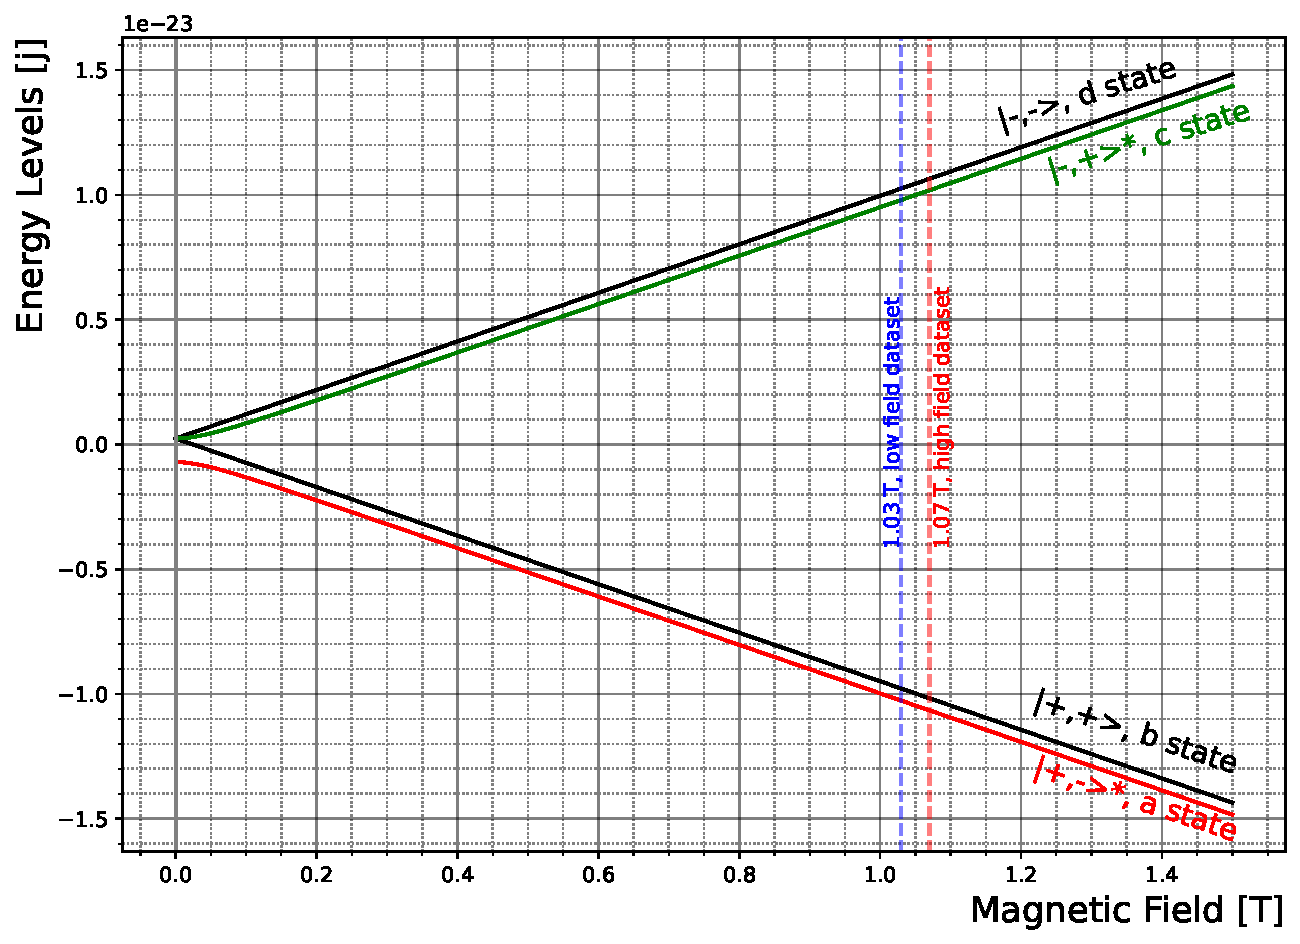
\includegraphics[width = \textwidth]{figures/chapter 3/HyperfineLevels.pdf}
\caption{Zeeman plot of the 4 hyperfine Levels of the 1s state. The blue and red dotted lines denote the magnetic field configuration corresponding to the two dataset used for the measurement. Each of the four lines is labeled accordingly to its spin configuration at high magnetic field regime. The d and b states correspond exactly to the parallel and antiparallel spin alignments (up-up and down-down) for the antiproton and positron. The c state and a state are mixed due to the presence of the external magnetic field, and only in the high field limit the states correspond to the up-down or down-up spin configuration.}\label{fig:ZeemanDiagram}
\end{figure}

As explained in the introduction \commento{richiamo all'introduzione}, the only trappable states are the c and d, which are the "low-field seeking" states. In high field regime, that is the case of the ALPHA experiment (magnetic field at $\simeq$ \SI{1}{\tesla}), the hyperfine splitting is defined as the frequency difference between the transition from the \textbf{d} state to the \textbf{a} state and the transition from the \textbf{c} state and the \textbf{b} state.

\begin{equation}
f_{da} - f_{cb}  = \left[(E_d - E_a) - (E_c - E_b)\right] \frac{1}{2 \pi \hbar} = \dfrac{A \hbar}{2 \pi} 
\end{equation}

it is important to highlight that this relation is valid only if the two transitions are measured at the same magnetic field value. This point is particularly significant, as it introduces one of the key characteristics of the magnetic field in the experiment. In fact, the large superconducting solenoid in alpha, the \textit{Carlsberg} magnet, produces a magnetic field that is affected by drift over time. The characterization of this drift is made through the ECR technique (\commento{reference}), which measure the magnetic field along z axis of the trap. The ECR measurement are reported in figure \ref{fig:ECR_term_bdrift}, that shows the magnetic field value measured at \SI{261.8}{\milli \meter} \commento{explain why at this location} at different time during the experiment. While the experimental protocol will be discussed later be discussed later, it is evident from the figure that there is an initial transient phase, during which the magnetic field remains constant or exhibits an upward drift (attributed to fine scale flux relaxation following the solenoid reset). This is followed by slower, long-term, downward linear drift of the field, due to decay of the of persistent currents in the external solenoid. The linear drift of the magnetic field is expected to be negative, causing a shift in the resonance of the transitions of about \SI{70}{\kilo \hertz \per \hour}. 

\begin{figure}[hbtp]
\centering
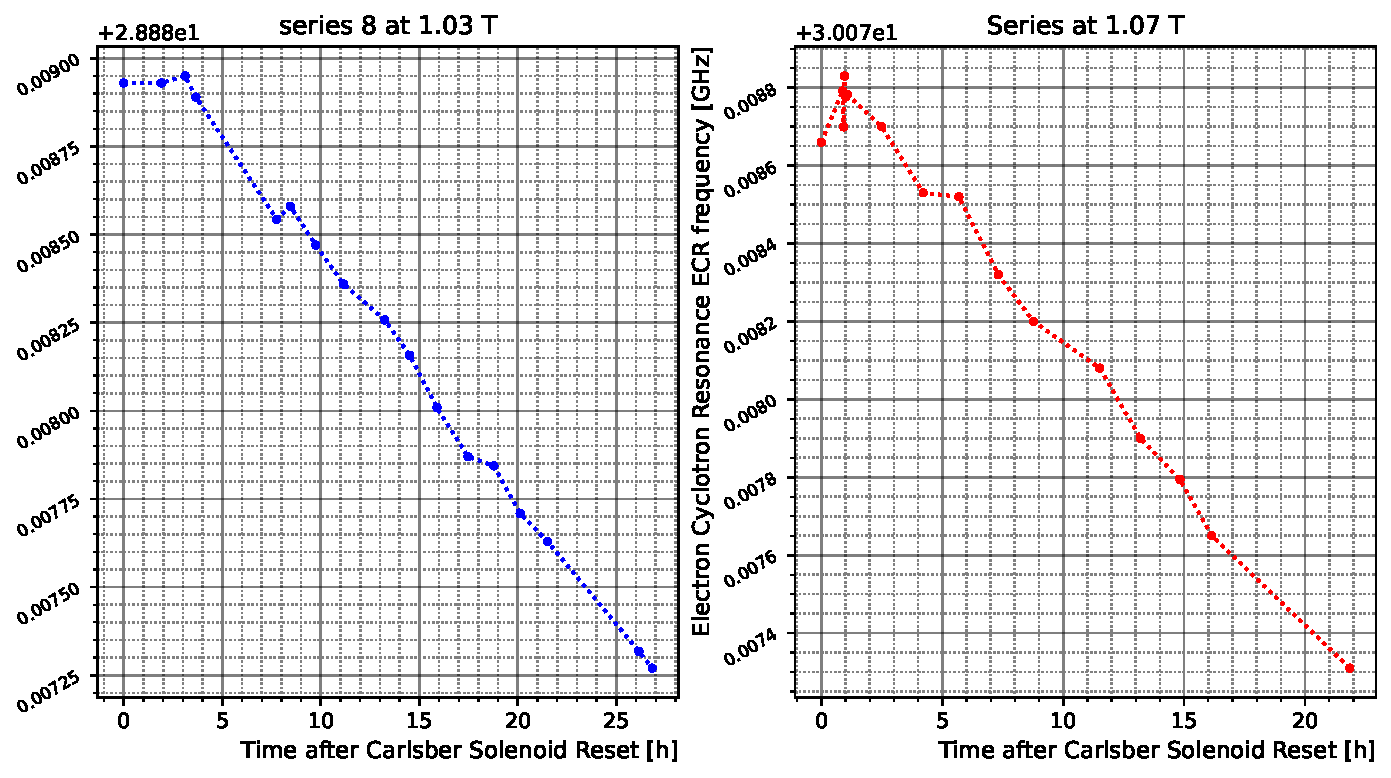
\includegraphics[width=\textwidth]{figures/chapter 3/ECR.pdf}
\caption{ECR measurement of the Magnetic field drift over time. The two series on points show the trend of the magnetic field over time from the most recent reset of the \textit{Carlsberg} superconducting solenoid, for the two dataset used for the measurement, which differ for a small offset of the magnetic field at the trap center ($\simeq$ \SI{0.04}{\tesla})}
\label{fig:ECR_term_bdrift}
\end{figure}

\section{Experimental Protocol}
\contentof{Description of the experimental protocol: stacking, measurement scan from lower to higher frequencies ecc. Things to mention are: 
\begin{itemize}
\item destructive measurement: depletion effects
\item Magnetic field profile
\item step duration, clearing...
\end{itemize}
}

This section provides a detailed description of the experimental protocol followed during data collection. The experimental data for spectroscopy measurement at ALPHA are constituted by looking at number of annihilating atoms over time. Depending on the different lines that the experiment aims to measure, various lasers, as the \SI{243}{ \nano \meter} for 1s-2s line, the \SI{121}{\nano \meter} for the Lyman-$\alpha$ or microwave light is used to kick-out atoms, which annihilate on the trap walls. The physics process involved can be different: for the 1s-2s spectroscopy ionization and momentum transfer from the laser light to the atoms plays the main role, while for the hyperfine measurement, the positron spin flip from a trappable to un-trappable state is the main physics mechanism for the ejection of atoms. To probe the \textbf{cb} and \textbf{da} transitions, microwave light is delivered into the trap environment via the wave guide depicted in figure \ref{fig:TrapScheme}. The frequency of the light is tuned between the range of \SI{28}{\giga \hertz}-\SI{31}{\giga \hertz}, selected based on the corresponding operating point from the the \SI{1}{\tesla} magnetic field. The experimental spectra are obtained by stacking antihydrogen atoms, approximately 1400-1600, in the \SI{0.5}{\kelvin} magnetic potential well. At first, these atoms are evenly split between the \textbf{c} and \textbf{d} states, while \textbf{b} and \textbf{a} states remain un-populated, since atoms produced in these states rapidly ($\simeq$ \SI{10}{\milli \second}) escapes and annihilates on the trap wall upon creation. After some magnets manipulation which creates the magnetic field suited for the measurement, that will be discussed later, the microwave light if finally injected at varying frequencies in increasing steps of \SI{5}{\kilo \hertz} each, with each step held constant for \SI{8}{\second}. The protocol used during the 2024 data taking comprises a number of 48 frequency steps, (total of \SI{240}{\kilo \hertz}), followed by an high power phase, named "clearing", consisting of 16 frequency steps of the same duration, during which residual \textbf{c} state or \textbf{d} states atoms that did not undergo transition are removed. This is the experimental procedure used to acquire a single spectra, corresponding to a \fcb or \fda transition, with the only difference of changing the microwave frequency about + \SI{1420390}{\kilo \hertz} to hit the first of the second transition. The data taking consisted of measuring in sequence \fcb and \fda, with a 300s pause in between during which the microwave system is switched off to cool down the electrodes of the trap. This procedure constitutes a single replicate, that was repeated for a of 8 times, constituting a set of data. Data were collected in two separate sets: one at \SI{1.03}{\tesla} and one at \SI{1.07}{\tesla} \commento{explain why this choice}, corresponding to different on-axis field minimum achieved by adjusting the target current in the Carlsberg solenoid. We will refer to these as low field and high field datasets, respectively.


\begin{figure}[hbtp]
\centering
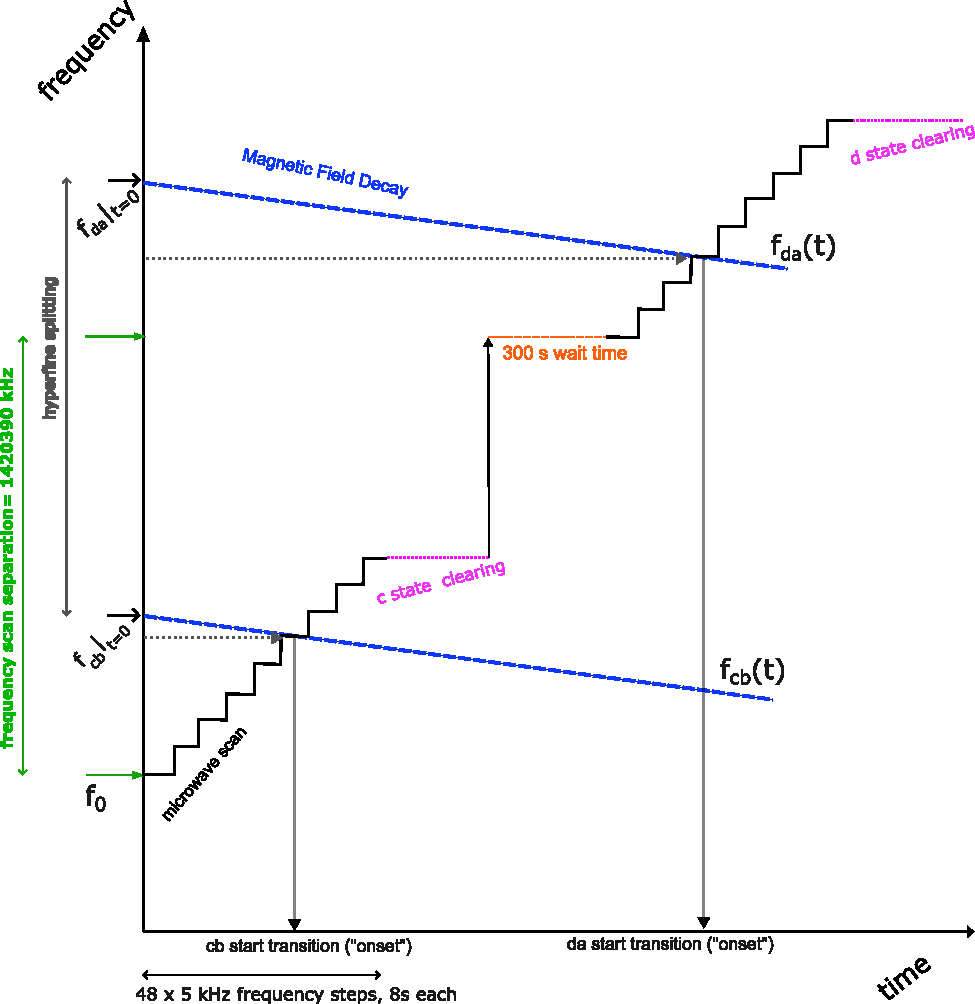
\includegraphics[width= 0.8\textwidth]{figures/chapter 3/SchemeBdrift.pdf}
\caption{Scheme of a single experimental repetition. Each dataset consists of 8 such repetitions, with atoms stacked between each run for the next cycle. The initial frequency $f_{0}$, the first microwave sweep of the \fcb scan, is determined by a low power scan to locate the "onset" of the transition. For subsequent repetitions, the starting frequency of each sweep is located is adjusted by subtracting the expected megnetic field drift.}
\end{figure}

It is important to clarify that, in this context, the experimental spectra refer to the annihilation counts recorded by the SVD over time. These spectra are influenced by the depletion of the total atomic population available during the microwave sweep, and are shaped by several others factors, as the temperature of the atom sample, the unknown standing wave pattern, Doppler broadening, magnetic field inhomogeneities and the natural linewidth of the transition. The interplay of all these effects collectively determines the observed spectral shape.


\subsection{Magnetic Field Profile}

Particular car has been dedicated in designing the magnetic field. The magnetic field was designed to reduce the second order derivative. The physical explanation is that in a "steep" magnetic field, the atoms crosses the magnetic field minimum rapidly, and this reduces the interaction time with the microwave field to induce transition.

\begin{figure}[hbtp]
\centering
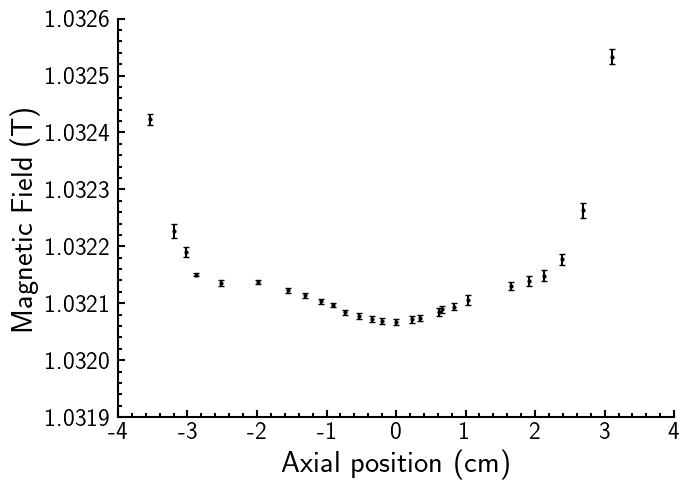
\includegraphics[width=0.75\textwidth]{figures/chapter 3/2024_MFF_DriftCorrected.png}
\caption{On-Axis magnetic field profile}
\end{figure}
 

\section{Microvawe System}
\contentof{Talk about the setup of the microwave system, issues with the energy distribution and not very well defined resonance, introduce the microvawe flat field for}

